\documentclass[border=10pt]{standalone}
\usepackage{tikz}
\usetikzlibrary{shapes.geometric, arrows, positioning, calc, fit, backgrounds}

% Define block styles using modern \tikzset
\tikzset{
    startstop/.style = {rectangle, rounded corners, minimum width=3.5cm, minimum height=0.8cm, text centered, draw=black, fill=red!20},
    io/.style = {trapezium, trapezium left angle=70, trapezium right angle=110, minimum width=3cm, minimum height=0.8cm, text centered, draw=black, fill=blue!15},
    process/.style = {rectangle, minimum width=4cm, minimum height=1cm, text centered, draw=black, fill=orange!20},
    heavy/.style = {rectangle, minimum width=4.5cm, minimum height=1cm, text centered, draw=black, fill=purple!20, line width=1pt},
    decision/.style = {diamond, aspect=2.5, minimum width=4cm, minimum height=1cm, text centered, draw=black, fill=green!20},
    arrow/.style = {thick,->,>=stealth}
}

\begin{document}

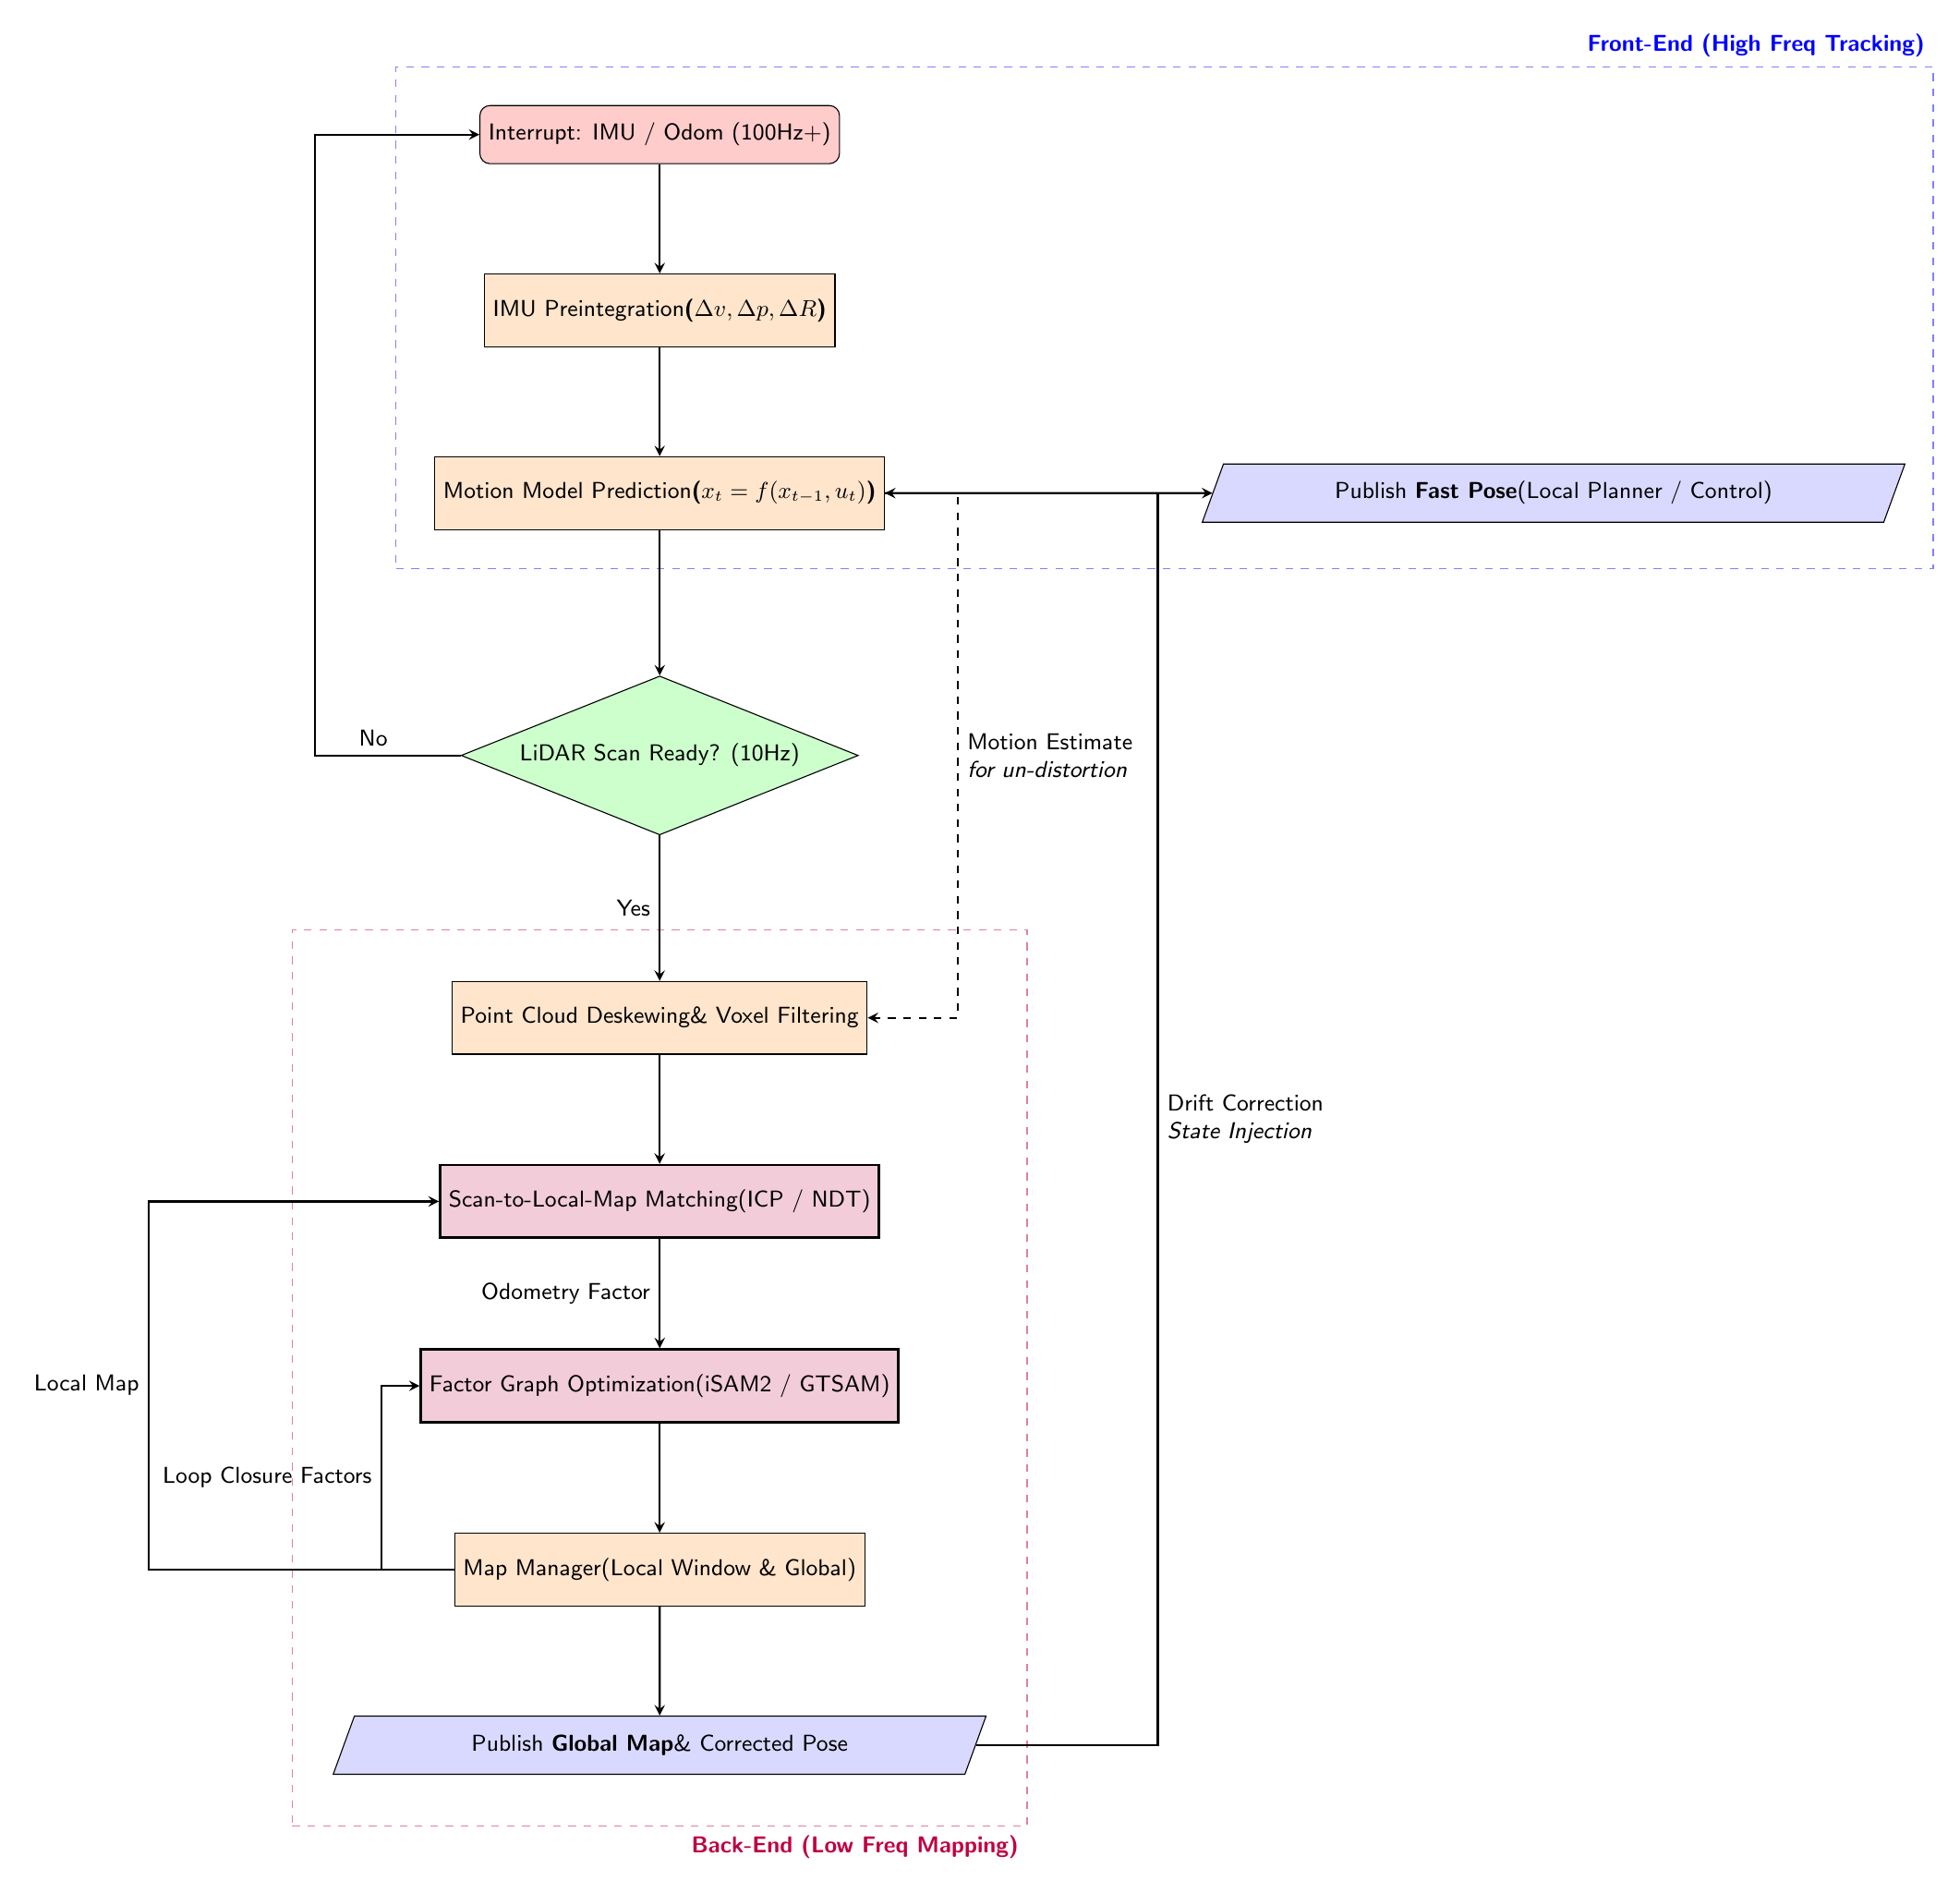
\begin{tikzpicture}[node distance=1.5cm, font=\sffamily\small]

% --- TRACKING FRONT-END (100Hz+) ---
\node (start) [startstop] {Interrupt: IMU / Odom (100Hz+)};
\node (preint) [process, below=of start] {IMU Preintegration \\ \textbf{($\Delta v, \Delta p, \Delta R$)}};
\node (predict) [process, below=of preint] {Motion Model Prediction \\ \textbf{($x_{t} = f(x_{t-1}, u_t)$)}};
\node (pub_fast) [io, right=of predict, xshift=3cm] {Publish \textbf{Fast Pose} \\ (Local Planner / Control)};

% --- THE GATEKEEPER & PRE-PROCESSING ---
\node (check) [decision, below=of predict, yshift=-0.5cm] {LiDAR Scan Ready? (10Hz)};
\node (deskew) [process, below=of check, yshift=-0.5cm] {Point Cloud Deskewing \\ \& Voxel Filtering};

% --- MAPPING BACK-END (Asynchronous) ---
\node (match) [heavy, below=of deskew] {Scan-to-Local-Map Matching \\ (ICP / NDT)};
\node (graph) [heavy, below=of match] {Factor Graph Optimization \\ (iSAM2 / GTSAM)};
\node (map) [process, below=of graph] {Map Manager \\ (Local Window \& Global)};
\node (pub_map) [io, below=of map] {Publish \textbf{Global Map} \\ \& Corrected Pose};

% --- CONNECTIONS ---

% Fast Loop (No LiDAR)
\draw [arrow] (start) -- (preint);
\draw [arrow] (preint) -- (predict);
\draw [arrow] (predict) -- (pub_fast);
\draw [arrow] (predict) -- (check);
\draw [arrow] (check.west) -- node[anchor=south, xshift=-0.2cm] {No} ++(-2cm,0) |- (start.west);

% Slow Loop (With LiDAR)
\draw [arrow] (check) -- node[anchor=east] {Yes} (deskew);
\draw [arrow] (deskew) -- (match);
\draw [arrow] (match) -- node[anchor=east] {Odometry Factor} (graph);
\draw [arrow] (graph) -- (map);
\draw [arrow] (map) -- (pub_map);

% Deskewing connection (Frontend aids deskewing)
\draw [arrow, dashed] (predict.east) -- ++(1cm,0) |- (deskew.east)
    node[pos=0.25, anchor=west, align=left] {Motion Estimate \\ \textit{for un-distortion}};

% Feedback Loops
\draw [arrow] (pub_map.east) -- ++(2.5cm,0) |- (predict.east) 
    node[pos=0.25, anchor=west, align=left] {Drift Correction \\ \textit{State Injection}};

\draw [arrow] (map.west) -- ++(-4.2cm,0) |- (match.west) 
    node[pos=0.25, anchor=east] {Local Map};

\draw [arrow] (map.west) -- ++(-1cm,0) |- (graph.west) 
    node[pos=0.25, anchor=east] {Loop Closure Factors};

% --- BOUNDARY BOXES ---
\begin{scope}[on background layer]
    % Front-End Box
    \node[draw, dashed, blue!50, inner sep=15pt, fit=(start) (pub_fast) (predict) (preint), 
          label={[anchor=south east, blue]north east:\textbf{Front-End (High Freq Tracking)}}] (frontend) {};
    
    % Back-End Box
    \node[draw, dashed, purple!50, inner sep=20pt, fit=(match) (pub_map) (deskew), 
          label={[anchor=north east, purple]south east:\textbf{Back-End (Low Freq Mapping)}}] (backend) {};
\end{scope}

\end{tikzpicture}

\end{document}